\part{Conservation}
\lecture{Conservation}{Conservation}
\section{Conservation}

\title{Ordinary Differential Equations}
\subtitle{Math 232 - Week 3, Day 1}
\date{9 Sep 2013}

\begin{frame}
  \titlepage
\end{frame}

\begin{frame}
  \frametitle{Outline}
  \tableofcontents[currentsection]

  Section 2.4 of the book.
\end{frame}


\subsection{Mixing Problems}


\begin{frame}
  \frametitle{Example}

  {\color{red}Brine is pumped into a tank at 50 liters per hour and has .5 kg per
  liter of salt.} {\color{blue}The volume of the tank is 500 liters, and initially
  the tank contains pure water.} {\color{purple}The well mixed solution is pumped out
  at 50 liters per hour.}

  What is the concentration of the solution in the tank at any time?

\end{frame}


\begin{frame}{Collect the Given Information}

  \only<1>{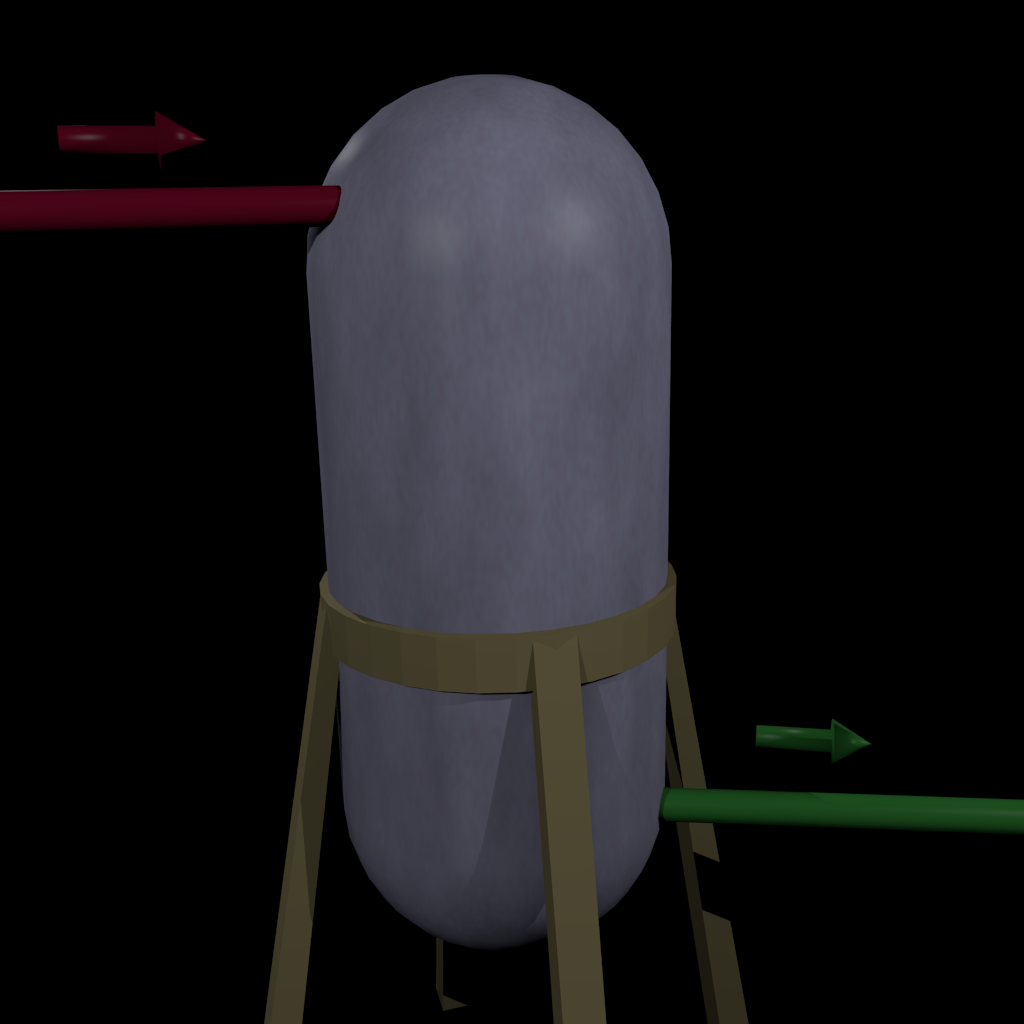
\includegraphics[width=8cm]{img/singleTank}}
  \only<2>{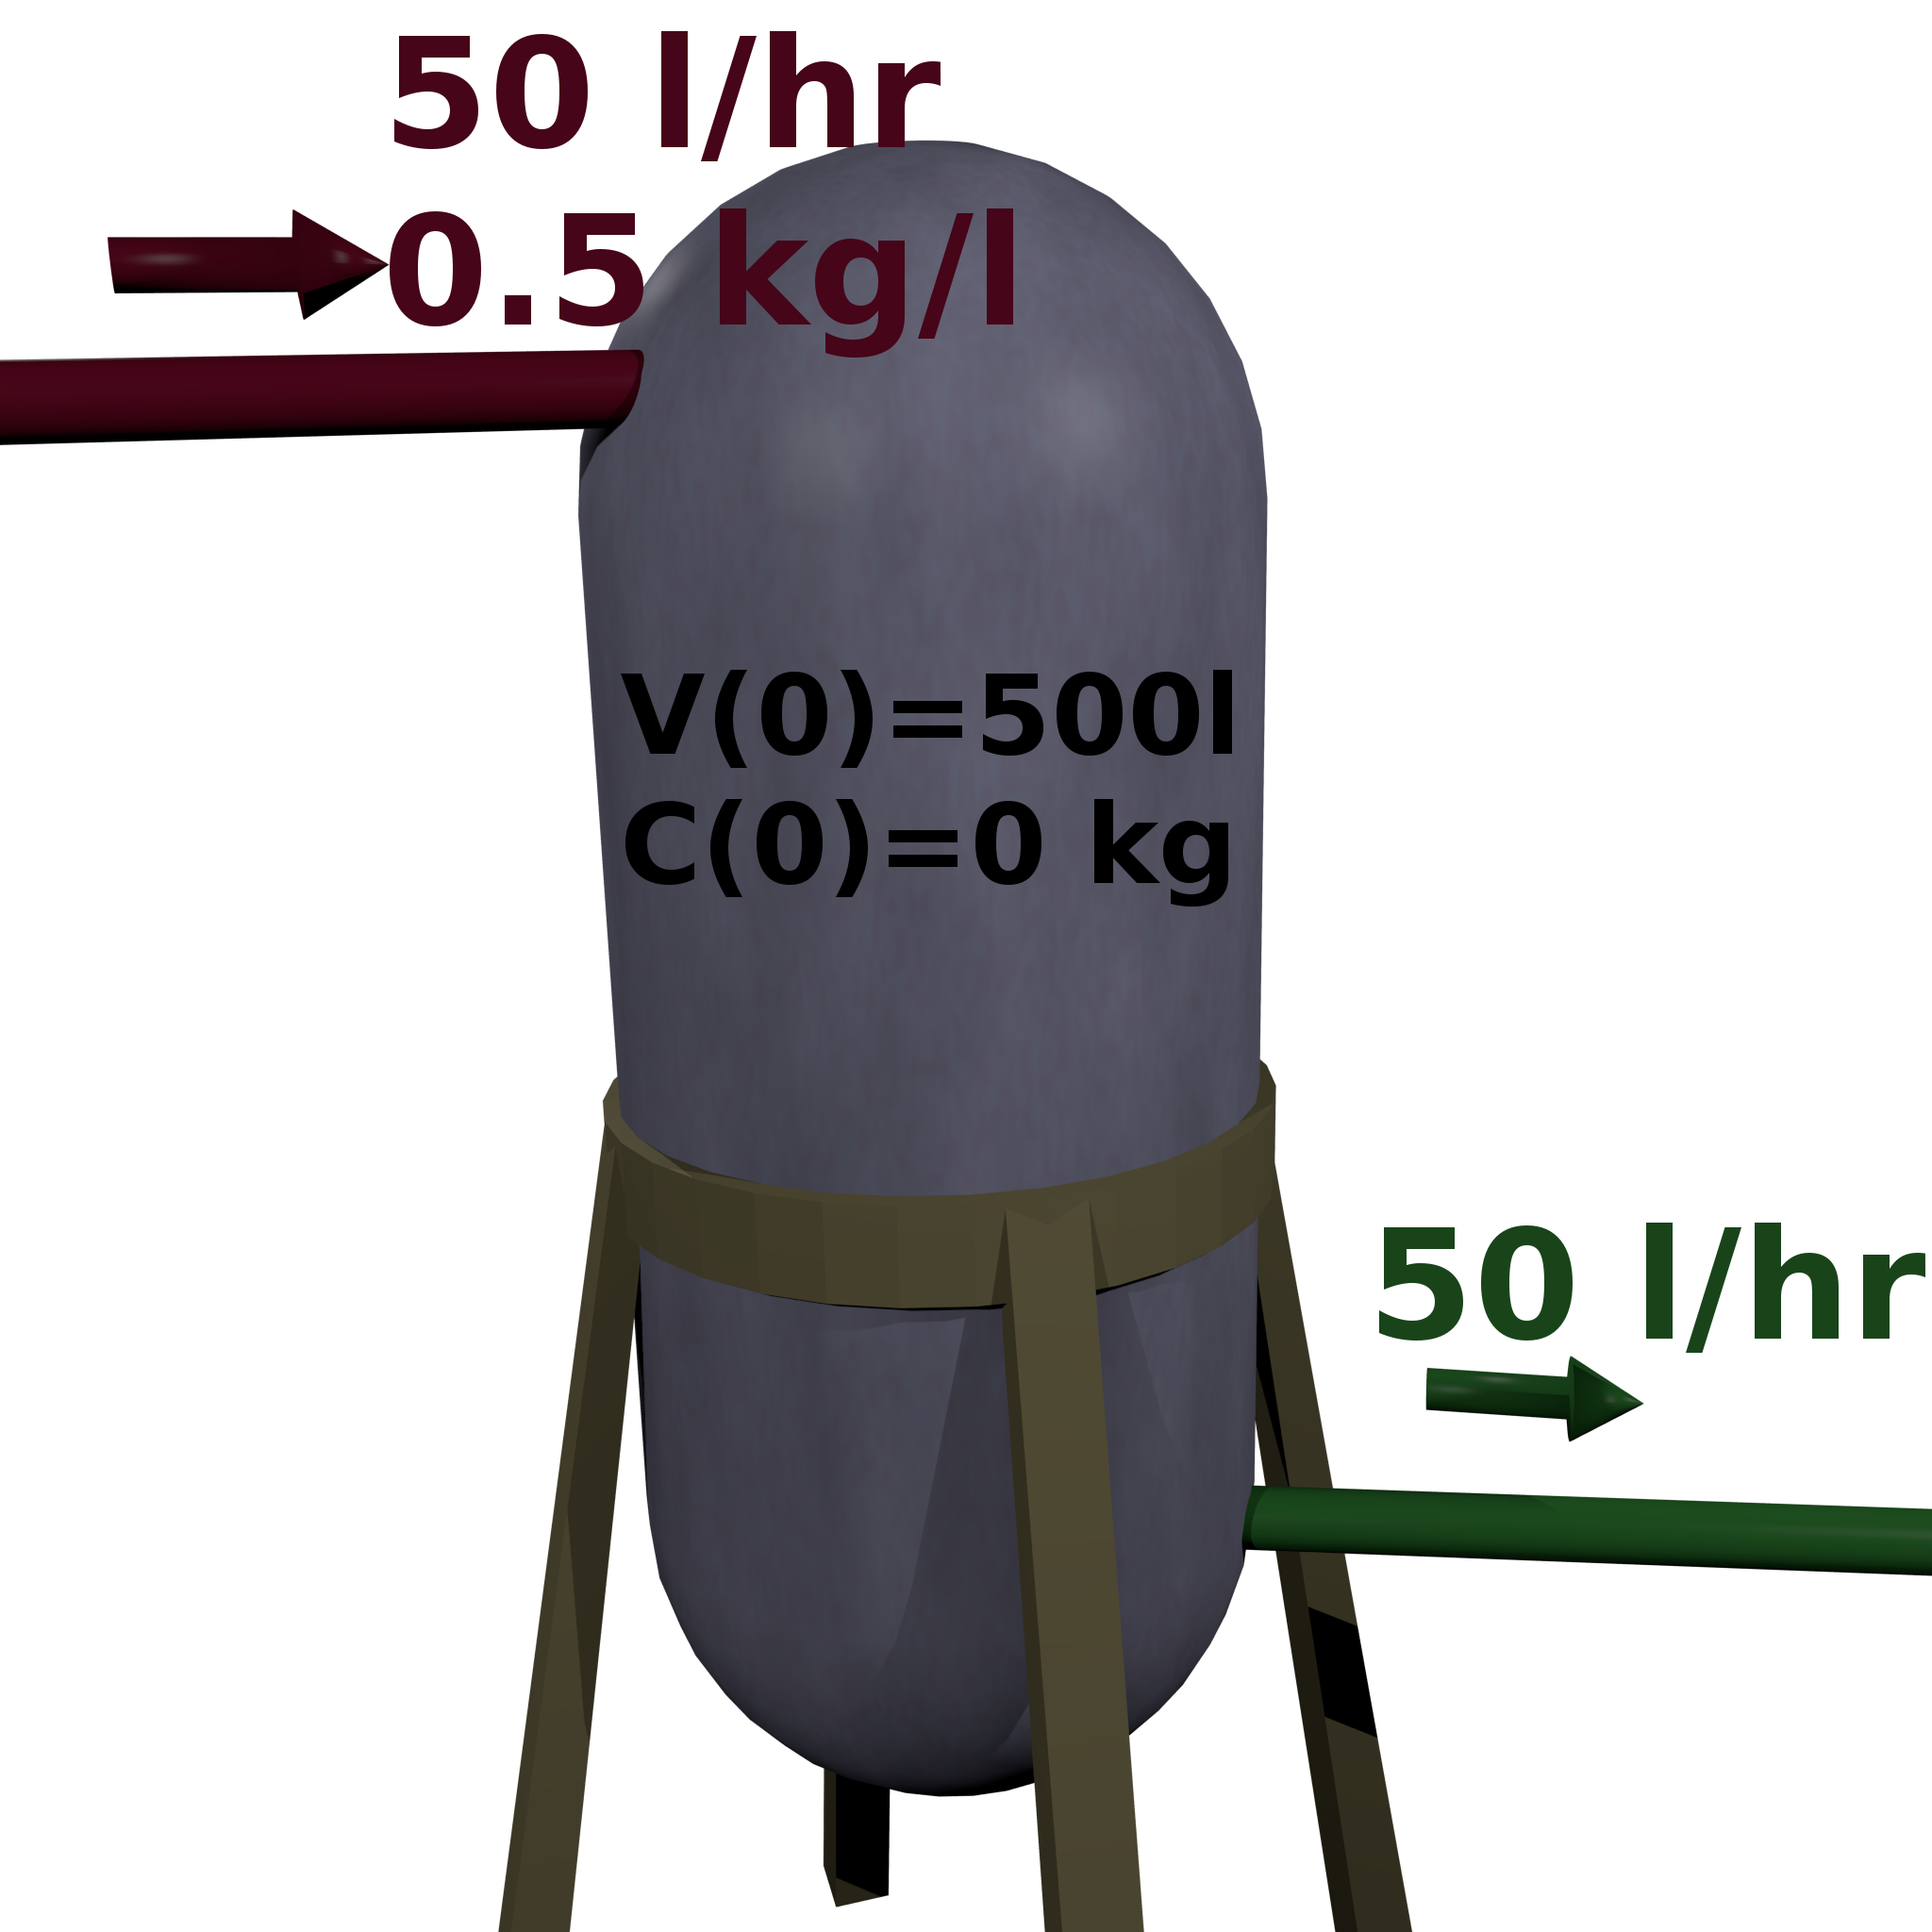
\includegraphics[width=8cm]{img/singleTankAnnotated}}
  
\end{frame}

\begin{frame}
  \frametitle{Conservation of Mass}

  Mass is conserved.

  \uncover<2->{Let $A(t)$ be the amount of ``stuff'' in the tank (kg).}

  \uncover<3->{

    \begin{eqnarray*}
      \Rightarrow ~ \frac{dA}{dt} & = & \mathrm{{\color{red}Rate ~ it ~ changes} ~
        (kg/hr)} \\
      & = & \mathrm{{\color{red}rate ~ in ~ - ~ rate ~ out}}.
    \end{eqnarray*}

  }

\end{frame}


\begin{frame}

  \begin{eqnarray*}
    \mathrm{rate~in~kg/hr} & = & \uncover<2->{.5 \frac{kg}{l} \cdot 50 \frac{l}{hr} \\
    & = & 25 \frac{kg}{hr}}
  \end{eqnarray*}

  \uncover<3->{

    \begin{eqnarray*}
      \mathrm{rate~out~kg/hr} & = & \uncover<4->{A(t)~kg \cdot
        \frac{1}{500~l} \cdot 50 \frac{l}{hr} \\
        & = & \frac{1}{10}A(t)}
    \end{eqnarray*}

  }

  \uncover<5->{

    \begin{eqnarray*}
      A'(t) & = & 25 - \frac{1}{10} A(t), \\
      A(0) & = & 0
    \end{eqnarray*}

  }

\end{frame}


\begin{frame}

  \begin{eqnarray*}
    \frac{1}{25 - \frac{1}{10}A} A' & = & 1, \\
    \int \frac{1}{25 - \frac{1}{10}A} A' ~ dt & = & \int 1 ~ dt, \\
    -10 \ln\lp25 - \frac{1}{10}A\rp & = & t + c \\
     \ln\lp25 - \frac{1}{10}A\rp & = & -\frac{t + c}{10} \\
     25 - \frac{1}{10} A & = & ke^{-t/10}, \\
     A & = & 250 - 10ke^{-t/10}, \\
     A(0) & = & 0 \\
     & = & 250-10k, \\
     k & = & 25, \\
     A(t) & = & 250-250e^{-t/10}
  \end{eqnarray*}

\end{frame}

\begin{frame}

  Concentration:
  \begin{eqnarray*}
    C(t) & = & A(t)/500 \\
    & = & \frac{1}{2} - \frac{1}{2} e^{-t/10}.
  \end{eqnarray*}

\end{frame}

\begin{frame}
  \frametitle{Example}

  {\color{red}A 2000 liter tank initially contains water with a solution of 0.2 kg
  per liter of salt.} {\color{blue} Brine is pumped in at a rate of 100 liters per
  hour with a concentration of 0.3 kg per liter.} {\color{purple}The well mixed
  solution is pumped out at a rate of 100 liters per hour.} Determine
  the amount of salt in the tank at any time.

  \vspace{1cm}
  Let $A(t)$ be the amount of salt in the tank at time $t$.
\end{frame}


\iftoggle{clicker}{%
\begin{frame}
  \frametitle{Clicker Quiz}
    
      \ifnum\value{clickerQuiz}=1{%

        What is the rate that salt flows into the tank?

       \vfill

       \begin{tabular}{l@{\hspace{3em}}l}
         A: & 10000 kg/hr. \\
         B: & 333.33 kg/hr. \\
         C: & 30 kg/hr. \\
         D: & 0.3 kg/hr. \\ 
       \end{tabular}

     }\fi

     \ifnum\value{clickerQuiz}=2{%

        What is the rate that salt flows into the tank?

       \vfill

       \begin{tabular}{l@{\hspace{3em}}l}
         A: & 10000 kg/hr. \\
         B: & 333.33 kg/hr. \\
         C: & 30 kg/hr. \\
         D: & 0.3 kg/hr. \\ 
       \end{tabular}


     }\fi

      \ifnum\value{clickerQuiz}=3{%
    What is the rate that salt flows into the tank?

       \vfill

       \begin{tabular}{l@{\hspace{3em}}l}
         A: & 10000 kg/hr. \\
         B: & 333.33 kg/hr. \\
         C: & 30 kg/hr. \\
         D: & 0.3 kg/hr. \\
       \end{tabular}

     }\fi

    \vfill
    \vfill
    \vfill

\end{frame}

}


\iftoggle{clicker}{%
\begin{frame}
  \frametitle{Clicker Quiz}
    
      \ifnum\value{clickerQuiz}=1{%

        What is the rate that salt flows out of the tank?

       \vfill

       \begin{tabular}{l@{\hspace{3em}}l}
         A: & A/20  kg/hr. \\
         B: & A/100 kg/hr. \\
         C: & 1/20  kg/hr. \\
         D: & 100   kg/hr. \\ 
       \end{tabular}

     }\fi

     \ifnum\value{clickerQuiz}=2{%

        What is the rate that salt flows out of the tank?

       \vfill

       \begin{tabular}{l@{\hspace{3em}}l}
         A: & A/20  kg/hr. \\
         B: & A/100 kg/hr. \\
         C: & 1/20  kg/hr. \\
         D: & 100   kg/hr. \\ 
       \end{tabular}

     }\fi

      \ifnum\value{clickerQuiz}=3{%
        What is the rate that salt flows out of the tank?

       \vfill

       \begin{tabular}{l@{\hspace{3em}}l}
         A: & A/20  kg/hr. \\
         B: & A/100 kg/hr. \\
         C: & 1/20  kg/hr. \\
         D: & 100   kg/hr. \\
       \end{tabular}


     }\fi

    \vfill
    \vfill
    \vfill

\end{frame}

}



\begin{frame}

  Let $A(t)$ be the amount of salt in the tank at time $t$.

  \begin{eqnarray*}
    A' & = & \mathrm{rate~in~} - \mathrm{~rate~out}.
  \end{eqnarray*}

  \begin{eqnarray*}
    \mathrm{rate~in} & = & 100 \frac{l}{hr} \cdot .3 \frac{kg}{l} \\
    & = & 30 \frac{kg}{hr}
  \end{eqnarray*}

  \begin{eqnarray*}
    \mathrm{rate~out} & = & A ~ kg \cdot \frac{1}{2000 l} \cdot 100 \frac{l}{hr} \\
    & = & \frac{1}{20} A
  \end{eqnarray*}

\end{frame}

\begin{frame}
   
  \begin{eqnarray*}
    A' & = & 30 - \frac{1}{20} A, \\
    A(0) & = & 2000 l \cdot .2 \frac{kg}{l} \\
    & = & 400 ~ kg
  \end{eqnarray*}

\end{frame}


\begin{frame}

  \begin{eqnarray*}
    A' + \frac{1}{20} A & = & 30 \\
    \uncover<2->{
      A' e^{t/20} + \frac{1}{20} e^{t/20} A & = & 30 e^{t/20} \\
      \frac{d}{dt} \lp A e^{t/20} \rp  & = & 30 e^{t/20} \\
      A e^{t/20}  & = & 600 e^{t/20} + C \\
      A  & = & 600 + C e^{-t/20} \\
      A(0) & = & 400 \\
      & = & 600 + C \\
      \Rightarrow C & = & -200 \\
      A(t) & = & 600-200 e^{-t/20}
    }
  \end{eqnarray*}

\end{frame}


\begin{frame}
  \frametitle{Example}

  {\color{red}A 500 liter tank is initially full and contains fresh water.} 
  {\color{blue}Brine with a concentration of 0.1 kg per liter is pumped into 
  the tank at a rate of 20 liters per hour.} {\color{purple}The well mixed 
  solution is pumped out at a rate of 30 liters per hour.}  
  What will the concentration be at the moment the tank is half full?

\end{frame}


\begin{frame}

  \begin{eqnarray*}
    A' & = & \mathrm{rate~in~} - \mathrm{~rate~out}
  \end{eqnarray*}

  \begin{eqnarray*}
    \mathrm{Rate~in} & = & .1 \frac{kg}{l} \cdot 20 \frac{l}{hr} \\
    & = & 2 \frac{kg}{l}
  \end{eqnarray*}

  \begin{eqnarray*}
    v(t) & = & 500-10t
  \end{eqnarray*}

  \begin{eqnarray*}
    \mathrm{rate~out} & = & A kg \cdot \frac{1}{500-10t ~ l} \cdot 30 \frac{l}{hr} \\
    & = & A \frac{30}{500-10t}
  \end{eqnarray*}

  \begin{eqnarray*}
    A' & = & 2 - A \frac{30}{500-10t}
  \end{eqnarray*}

\end{frame}


\begin{frame}

  \begin{eqnarray*}
    A' + A \frac{30}{500-10t} & = & 2 \\
    (500-10t)^{-3} A' + 30(500-10t)^{-4} A & = & 2 (500-10t)^{-3} \\
    \frac{d}{dt} \lp (500-10t)^{-3} A \rp & = & 2 (500-10t)^{-3} \\
    (500-10t)^{-3} A  & = & \int 2 (500-10t)^{-3} ~ dt  \\
    (500-10t)^{-3} A  & = & \frac{1}{10} (500-10t)^{-2} + C  \\
    A(0) & = & 0 \\
    & = & \frac{1}{10} 500^{-2} + C \\
    C & = & -\frac{1}{10\cdot500^{2}}
  \end{eqnarray*}

  \begin{eqnarray*}
    A(t) & = & \frac{1}{10} (500-10t) - \frac{1}{10\cdot500^{2}} (500-10t)^3
  \end{eqnarray*}

\end{frame}


\begin{frame}

  The tank is half full when the volume is 250l:
  \begin{eqnarray*}
    v(t) & = & 250 \\
    250 & = & 500-10t \\
    \Rightarrow t & = & 25.
  \end{eqnarray*}

  \begin{eqnarray*}
    A(25) & = & \frac{1}{10} (500-10\cdot 25) - \frac{1}{10\cdot500^{-2}} (500-10\cdot 25)^3 \\
    & \approx & 18.75 ~ kg
  \end{eqnarray*}

  \begin{eqnarray*}
    \mathrm{Concentration} & = & A(25)/250 \\
    & \approx & 0.075 kg/l
  \end{eqnarray*}

\end{frame}

\subsection{Newton's Law of Cooling}

\begin{frame}
  \frametitle{Newton's Law of Cooling}

  {\color{red}The rate of change of the temperature of an object is 
  proportional to the difference between the temperature of the 
  object and the temperature of the surroundings.}

  Let M be the ambient (the surroundings) temperature.  

  Let $T(t)$ be the temperature of the object at time $t$. 

  \begin{eqnarray*}
    T'(t) & = & k (M-T)
  \end{eqnarray*}


\end{frame}

\subsection{Examples of Newton's Law of Cooling}

\begin{frame}
  \frametitle{Example}

  {\color{red}A brick is pulled out of a furnace and is 350 degrees Celsius.} 
  {\color{blue}It is placed outside where the air temperature is 20 degrees Celsius.} 
  {\color{purple}After one hour the temperature of the brick is 280
    degrees Celsius.}  
  What will the temperature of the brick be after 6 hours from when it
  was first pulled out of the furnace?

  \uncover<2->{
    
    \begin{eqnarray*}
      T' & = & k(M-T) \\
      T(0) & = & 350 \\
      M & = & 20 \\
      T(1) & = & 280 \\
      T(6) & = & ??
    \end{eqnarray*}

  }

\end{frame}


\begin{frame}

  \begin{eqnarray*}
    T' & = & k (20-T) \\
    \frac{T'}{20-T} & = & k \\
    -\ln(T-20) & = & kt + C,  \text{since} T > 20\\
    T & = & 20 + A e^{-kt}
  \end{eqnarray*}

  \begin{eqnarray*}
    T(0) & = & 350 \\
    & = & 20 + A \\
    A & = & 330, \\
    T(t) & = & 20 + 330 e^{-kt}
  \end{eqnarray*}

\end{frame}


\begin{frame}

  \begin{eqnarray*}
    T(1) & = & 280 \\
    & = & 20 + 330 e^{-k} \\
    k & = & -\ln\lp\frac{26}{33}\rp \\
    T(t) & = & 20 + 330 e^{t\ln\lp\frac{26}{33}\rp}
  \end{eqnarray*}

  \begin{eqnarray*}
    T(6) & = & 20 + 330 e^{6\ln\lp\frac{26}{33}\rp} \\
    & \approx & 98.9 ~C
  \end{eqnarray*}

\end{frame}


\begin{frame}
  \frametitle{Example}

  A cup of coffee is found. {\color{red}The temperature when it is found is 70
  degrees Celsius.} {\color{blue}Thirty minutes later its temperature is 65 degrees
  Celsius.} {\color{purple}The temperature in the room is 18 degrees Celsius.} 
  {\color{orange}When the coffee was poured the temperature was 85 degrees Celsius.} 
  When was the coffee poured?

  \uncover<2->{
    
    \begin{eqnarray*}
      t_0 & = & \mathrm{time~when~the~coffee~was~found.} \\
      M & = & 18 \\
      T(0) & = & 85   \\
      T(t_0) & = & 70 \\
      T(t_0+30) & = & 65.
    \end{eqnarray*}

  }

\end{frame}


\begin{frame}

  \begin{eqnarray*}
    T' & = & k(18-T) \\
    \frac{T'}{18-T} & = & k \\
    -\ln(T-18) & = & kt + C \\
    T & = & 18 + A e^{-kt} 
  \end{eqnarray*}

\end{frame}

\begin{frame}

  At time $t_0$:
  \begin{eqnarray*}
    T(t_0) & = & 70 \\
    & = & 18 + Ae^{-kt_0} \\
    \Rightarrow Ae^{-kt_0} & = & 52
  \end{eqnarray*}

  At time $t_0+30$:
  \begin{eqnarray*}
    A(t_0+30) & = & 65 \\
    & = & 18 + A e^{-kt_0-30k} \\
    & = & 18 + A e^{-kt_0} e^{-30k} \\
    & = & 18 + 52 e^{30k} \\
    \Rightarrow k & = & -\frac{1}{30} \ln\lp\frac{47}{52}\rp.
  \end{eqnarray*}

\end{frame}


\begin{frame}

  \begin{eqnarray*}
    T(0) & = & 85 \\
    & = & 18 + A e^{0} \\
    \Rightarrow A & = & 67
  \end{eqnarray*}

  \begin{eqnarray*}
    T(t)  & = & 18 + 67 e^{\frac{t}{30} \ln\lp\frac{47}{52}\rp} \\
    T(t_0)& = & 70 \\
    & = & 18 + 67 e^{\frac{t_0}{30} \ln\lp\frac{47}{52}\rp} \\
    \Rightarrow t_0 & = & \frac{30\ln\lp\frac{52}{67}\rp}{\ln\lp\frac{47}{52}\rp}.
  \end{eqnarray*}

\end{frame}



% LocalWords:  Clarkson pausesection hideothersubsections
